\chapter{从白皮书到研究计划}
\label{chap:22}

\begin{chapteropening}
量子天文学的研究计划要能执行，也要能失败。路线图需要写清观测量、数据产品、误差预算、里程碑和风险登记；读者应能把这一章直接改写成 proposal 的工作包、验收指标和失败判据。现代强度干涉白皮书、Cherenkov 阵列结果、谱复用方案、Type Ia 距离模型、量子网络望远镜设想和开放数据工具，把可做的近期工作和还需要 pathfinder 的远期工作分开 \citep{1956Natur.178.1046H,1974iiia.book.....H,2003RPPh...66..789M,2018SPIE10548E..1KO,2026arXiv260212717K,2017ICRC...35..828K,2019ICRC...36..714K,2020NatAs...4.1164A,2024MNRAS.529.4387A,2025PhRvD.111h3047K,2023PhRvL.130p0801M,2026PhRvA.113a2608P}。
\end{chapteropening}

\section{2026 到 2030：怎样把强度干涉做成常规数据产品}

近期目标是把已经可行的强度干涉变成可重复的数据产品，量子网络望远镜仍属于后续阶段。这个阶段的主要观测量是 \(\hat g^{(2)}_{ab}(\tau)\)、\(|V_{ab}|^2\)、目标光子率、零基线对比度、背景稀释因子和每条基线的协方差。VERITAS 和 MAGIC 已经证明 IACT 阵列可以做亮星强度干涉，\(\beta\) UMa 和 \(\gamma\) Cas 的结果显示，恒星角直径、快速自转和非球对称模型已经进入真实科学阶段 \citep{2020NatAs...4.1164A,2024MNRAS.529.4387A,2024ApJ...966...28A,2025ApJ...995..191A}。小口径 Sirius 演示和 AQuEye/IquEye 方案说明，教学实验、路径验证和大设施观测可以共用同一套事件表和相关器语言 \citep{2016SPIE.9907E..0NZ,2025MNRAS.537.2527M}。

近期项目的成熟度要写成可验收指标，不能停在“探测器可用”或“望远镜足够大”：
\begin{equation}
  \bm{r}=
  \left(
  \frac{R_\gamma}{R_{\rm req}},
  \frac{\sigma_{t,{\rm req}}}{\sigma_t},
  \frac{\beta_0}{\beta_{\rm req}},
  \frac{\sigma_{{\rm sys,req}}}{\sigma_{\rm sys}},
  \frac{N_{\rm cal}}{N_{{\rm cal,req}}}
  \right).
  \label{eq:ch22-readiness-vector}
\end{equation}
\begin{formulaexplain}[公式 (22.1) 解读]
\(\bm r\) 是项目成熟度向量，每一项都是实际能力与需求的比值。只有光子率、计时、对比度、系统误差和校准样本同时达标，近期项目才算闭合。
\end{formulaexplain}
\(R_\gamma\) 是每台望远镜的有效光子率，单位 \({\rm s}^{-1}\)；\(\sigma_t\) 是相对时间同步误差，单位 ps 或 ns；\(\beta_0\) 是零基线相关对比度，无量纲；\(\sigma_{\rm sys}\) 是校准后的系统误差地板；\(N_{\rm cal}\) 是可用校准星或校准观测数。若 \(R_\gamma/R_{\rm req}>1\) 但 \(\sigma_{\rm sys}\) 比目标 \(|V|^2\) 信号还大，项目仍然不成熟。强度干涉阵列研究反复强调，基线长度、\(u,v\) 覆盖、背景控制和零基线校准要一起闭合 \citep{2006ApJ...649..399L,2013APh....43..331D,2022MNRAS.512.1722K}。

\begin{figure}[tbp]
\centering
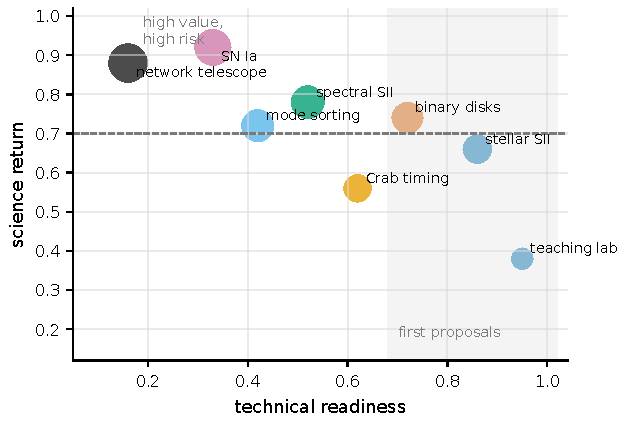
\includegraphics[width=0.86\linewidth]{figures/generated/chapter_22/ch22_roadmap_trade_space.pdf}
\caption{路线图中的技术成熟度、科学回报、成本和风险。右上方但成熟度较高的任务适合写成近期 proposal；左上方的任务有高科学价值但需要先做路径验证。点大小表示成本压力，位置表示技术成熟度和科学回报的相对判断。}
\label{fig:ch22-trade-space}
\end{figure}

2026--2030 年的第一批论文应尽量具体。可执行题目可以写成“用四台 IACT 在 416 nm 附近测量 10--30 颗亮星角直径，并给出公开相关器和校准库”；也可以写成“用同一套 pipeline 比较双星、Be 星盘和快速自转星的 \(|V|^2\) 模型”。每篇论文都应发布事件表格式说明、相关器版本、time-shift null test、校准星表、基线几何和后验样本。这样即使部分目标没有检出，也能留下可复用的仪器知识。

\section{2030 到 2040：多通道事件表要多出什么}

中期目标是把“一个蓝光滤光片上的 \(|V|^2\)”扩展成多通道事件表。光谱分辨强度干涉可以比较谱线内外的角尺度；偏振分辨相关可以检查磁场几何、散射和强场辐射；皮秒级事件表可以把光子统计作为新的时域数据产品。谱复用的吸引力在于，每个光谱通道的相干时间变长，而多个通道又可以并行累加 SNR；但代价是数据率、通道间校准和色散模型变复杂 \citep{2021sf2a.conf..335L,2022MNRAS.512.1722K,2024MNRAS.529.4387A}。

多通道阶段的基本数据产品可以写成
\begin{equation}
  \bm{d}=
  \left\{
  H_{ab}^{\nu p}(\tau),
  \widehat{|V_{ab}^{\nu p}|^2},
  C_{\nu_i\nu_j}^{p_i p_j},
  \bm{\Sigma}
  \right\}.
  \label{eq:ch22-data-vector}
\end{equation}
\begin{formulaexplain}[公式 (22.2) 解读]
\(\bm d\) 是多通道阶段的数据产品集合。它不只包含 \(|V|^2\)，还包括延迟直方图、跨频/跨偏振协方差和完整协方差矩阵。
\end{formulaexplain}
\(H_{ab}^{\nu p}\) 是望远镜 \(a,b\)、频率通道 \(\nu\)、偏振通道 \(p\) 的延迟直方图；\(|V|^2\) 是校准后的空间相干观测量；\(C_{\nu_i\nu_j}^{p_i p_j}\) 是跨频或跨偏振协方差；\(\bm{\Sigma}\) 是这些数据之间的协方差矩阵。只写“多通道量子观测”还不够；这些量怎样存储、归一化和发布，决定项目是否已经到工程阶段。

\begin{figure}[tbp]
\centering
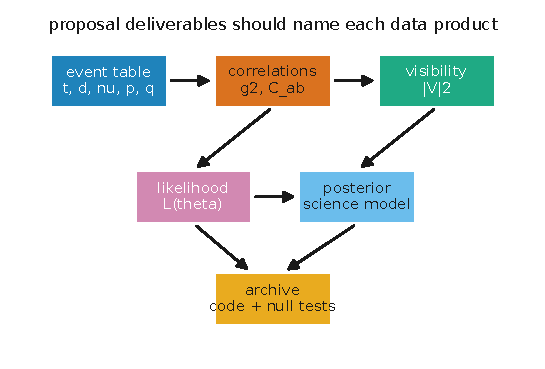
\includegraphics[width=0.88\linewidth]{figures/generated/chapter_22/ch22_data_product_stack.pdf}
\caption{从 proposal 到公开数据的产品链。事件表保留到达时间、望远镜、频率、偏振和质量标记；相关器把它变成 \(g^{(2)}\) 和协方差；空间模型给出 \(|V|^2\)；似然和后验连接到天体参数；归档要包含代码、版本和 null test。}
\label{fig:ch22-data-products}
\end{figure}

Type Ia 超新星距离是中期科学案例的典型高风险高回报项目。它需要快速触发、km 级到十 km 级基线、爆炸时间、速度模型、光球非球对称和强度干涉角半径联合建模。Kim、Nugent、Chen 和合作者的 toy model 给出了可行性边界：近邻、明亮、早期发现的事件才值得进入干涉跟进 \citep{2025PhRvD.111h3047K}。自然激光、Crab pulsar 光子统计、Be 星盘谱线和 AGN BLR 几何也可写成同一类计划，但每一个都要先说明触发率、可观测窗口、背景和失败判据。

\section{2040 以后：量子网络望远镜何时才是主线}

远期目标要分层写。本地模式排序和相位敏感测量不需要完整量子网络，也能提高小分离和亮度矩估计的信息效率 \citep{2016PhRvX...6c1033T,2017PhRvL.118g0801T}。two-photon astrometry、单光子辅助或线性光学 pathfinder 的目标，是把天文光和实验室量子资源稳定耦合 \citep{2023PhRvL.130p0801M,2024SPIE13095E..1NR}。纠缠辅助长基线干涉需要纠缠分发率、量子存储时间、频率转换效率、Bell fidelity 和天文同步共同达标，属于更后面的阶段 \citep{2025PhRvA.111d3701M,2025PhRvR...7d3278Z,2026PhRvA.113a2608P,2026Natur.651..326S}。

量子网络望远镜的资源门槛已经在第 \ref{chap:17} 章式 \eqref{eq:ch17-entanglement-rate}、\eqref{eq:ch17-memory-time} 和 \eqref{eq:ch17-effective-fidelity} 中写成链路率、存储时间和有效保真度的约束。proposal 要把同一组量放进验收表：\(R_{\rm ent}\) 是纠缠对产生率，单位 \({\rm s}^{-1}\)；\(\eta_{\rm link}\)、\(\eta_{\rm mem}\)、\(\eta_{\rm conv}\) 分别是链路、存储和频率转换效率；\(R_{\gamma,{\rm useful}}\) 是实际进入目标模式和时间窗的天文光子率；\(T_{\rm mem}\) 是可用存储时间；\(B/c\) 是基线光行时。\(B=1000\,{\rm km}\) 时 \(B/c\simeq3.3\,{\rm ms}\)，地面 km 级基线只需 \(\mu{\rm s}\) 到 ms 级同步，但全球或空间基线会把存储和分发压力迅速放大。链路损耗、存储退相干和有用光子率任何一项不达标，网络方案都还不足以替代常规强度干涉或振幅干涉。

\begin{figure}[tbp]
\centering
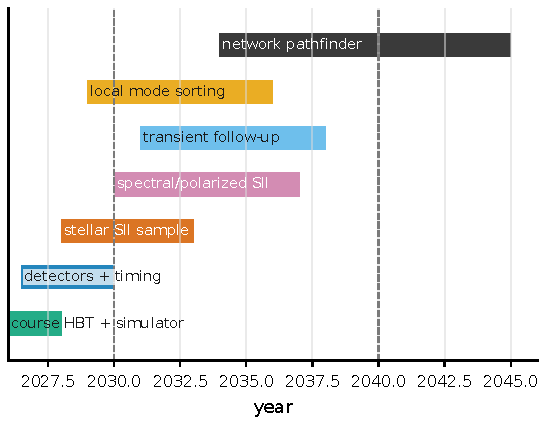
\includegraphics[width=0.92\linewidth]{figures/generated/chapter_22/ch22_program_timeline.pdf}
\caption{从课程 HBT 到量子网络 pathfinder 的阶段性时间线。绿色和蓝色任务建立人才、事件表、计时和校准；橙色和紫色任务产出第一代科学样本和多通道相关；黑色远期任务只有在本地模式排序、链路和存储指标达标后才应写成设施路线。}
\label{fig:ch22-timeline}
\end{figure}

\section{研究计划怎样写}

\Needspace{11\baselineskip}
一个可执行里程碑要把观测量和验收标准同时写清：
\begin{equation}
  m_j=
  \left(
  O_j,\,
  \sigma_{O,j}^{\rm goal},\,
  T_j,\,
  N_{{\rm null},j},\,
  D_{{\rm release},j}
  \right).
  \label{eq:ch22-milestone}
\end{equation}
\begin{formulaexplain}[公式 (22.3) 解读]
\(m_j\) 是第 \(j\) 个里程碑。它同时指定观测量、目标精度、时间、null test 数和发布数据，避免路线图只停在愿景。
\end{formulaexplain}
\(O_j\) 是观测量，例如 \(g^{(2)}(0)-1\)、\(|V|^2\)、谱线内外角尺度比或 \(D_A\)；\(\sigma_O^{\rm goal}\) 是目标精度；\(T_j\) 是完成日期或所需观测时间；\(N_{\rm null}\) 是要通过的 null test 数；\(D_{\rm release}\) 是要发布的数据产品。近期项目可以要求 \(N_{\rm null}\ge2\)：time-shift 和 off-source；中期多通道项目应要求 \(N_{\rm null}\ge4\)：time-shift、off-band、错偏振和注入恢复；远期网络项目还应包含链路保真度和存储退相干的独立验收。

\begin{figure}[tbp]
\centering
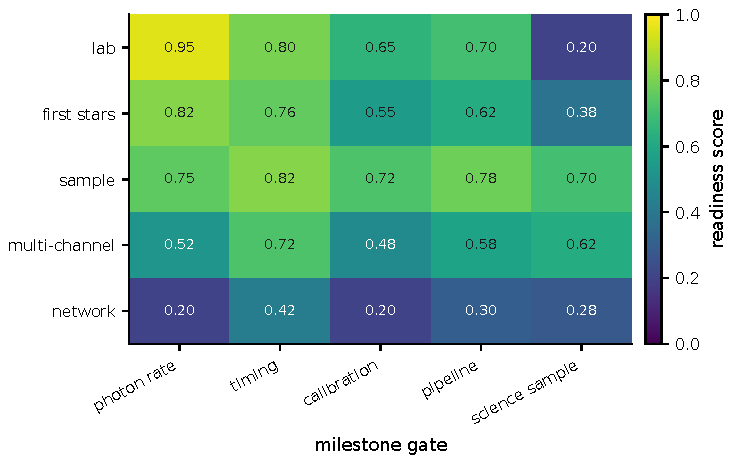
\includegraphics[width=0.92\linewidth]{figures/generated/chapter_22/ch22_milestone_gates.pdf}
\caption{不同阶段的里程碑门槛矩阵。课程实验和第一代恒星 SII 在光子率、计时和 pipeline 上已经较成熟，但多通道校准和网络阶段仍有明显缺口。数字只是 proposal 中应显式量化的 readiness score 示例，并不代表设施承诺。}
\label{fig:ch22-gates}
\end{figure}

误差预算要从第一版 proposal 就写清楚，并沿用第 \ref{chap:18} 章式 \eqref{eq:ch18-error-budget} 的分解。\(\sigma_{\rm stat}\) 来自 Poisson 或相关计数噪声；\(\sigma_{\rm cal}\) 来自零基线对比度、时间同步、偏振和光谱响应；\(\sigma_{\rm bg}\) 来自夜天光、连续谱或伴星背景；\(\sigma_{\rm model}\) 来自恒星盘、超新星光球、BLR 或 maser 几何；\(\sigma_{\rm sel}\) 来自触发、天气和目标选择。统计采样可以用 MCMC、nested sampling 或后验预测检查实现，但这些工具无法替代物理误差项本身 \citep{2013PASP..125..306F,2009MNRAS.398.1601F,1979ApJ...228..939C,2013ApJ...764..167S,2025ApJ...988...23P}。

\begin{figure}[tbp]
\centering
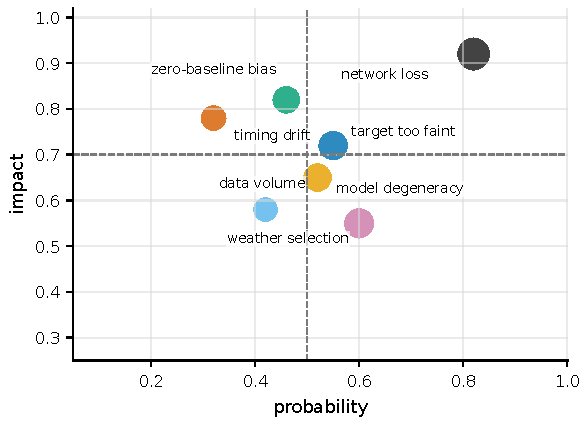
\includegraphics[width=0.86\linewidth]{figures/generated/chapter_22/ch22_risk_register.pdf}
\caption{路线图的风险登记图。右上角的风险需要在项目开始前配套缓解方案：例如网络损耗需要先做短基线 pathfinder，零基线偏差需要校准星库，目标过暗需要明确的触发和放弃标准。点越大表示缓解方案越弱。}
\label{fig:ch22-risk}
\end{figure}

风险登记表要和失败判据一起写。若目标星等比预期暗 1 mag，光子率下降到约 40\%；若系统误差地板停在 \(3\times10^{-5}\)，许多 \(|V|^2\) 小信号不再可测；若 Type Ia 触发晚 10 天，角半径更大但光度下降、模型不确定性上升；若网络链路每天只给很少高保真 entangled pairs，科学模式就应退回本地模式排序或强度干涉。路线图可以失败，但失败要告诉下一阶段该改什么。

\section{从课程项目怎样长成研究课题}

课程项目可以从第 \ref{chap:20} 章开始：桌面 HBT、事件表模拟、均匀圆盘拟合、SPADE Fisher 信息和假警报计算。较小的研究题目适合围绕一个 pipeline 展开，例如时间同步、相关器、校准库、目标样本或 open-data notebook。更完整的科学题目可以瞄准 Be 星 H\(\alpha\) 盘的谱线角尺度、快速自转星多基线模型、Crab pulsar 相位分辨光子统计、Type Ia 距离 toy model 的系统误差，或者本地模式排序和自适应光学的联合实验。大型合作项目再把这些课题接到 CTAO/IACT、ELT/VLTI/CHARA、Rubin、SKA、LIGO/Virgo/KAGRA/ET 或量子网络实验室。

一个项目至少要列出新增观测量、事件表字段、数据估计步骤、符号单位、典型范围、两个以上 null test，以及失败后仍能留下的数据、代码或仪器约束。这样的计划可以被复现、审查和改进；否则“量子”只停留在题目上。

